\documentclass[11pt]{article}
\usepackage{memo}

% Parmaters --
\title{\large\textbf{Creating and Using Post-Stratification Weighting for District-level Estimates}}
\author{\normalsize  Shiro Kuriwaki\thanks{Ph.D. Candidate, Department of Government and Institute of Quantitative Social Science, Harvard University. Thanks to Soichiro Yamauchi for helpful discussions.}}

\date{\normalsize October 2019}


\begin{document}
\maketitle

\onehalfspacing

In this memo I explore how representative CCES samples are at subnational geographies, and whether post-stratification weights ameliorate the problem. Although post-stratification weights are designed to coerce samples to be representative, one set of weights makes a sample representative to only one target, in CCES' case the entire U.S. It is not clear if those same weights \emph{also} make subgroup samples representative of their respective subgroup targets. 

Multi-level post-stratification (MRP) methods take another route, whereby the targets for granular joint distributions are computed first so that they can be combined to any preferred level of aggregation for the post-stratification step. However, MRP has several limitations. First, often times analysts only have marginal, not joint distributions at the level they care about. Second, one MRP model is specific to one outcome, so comparing more than one issue question would involve building as many multi-level models as there are outcomes. In contrast, once post-stratification weights are defined, it can be used for any sets of outcomes. 

\section{Post-stratification Weights and MRP}

Each method has its pros and cons, sumarized by the following table:

\begin{table}[!h]
\centering
\small
\begin{tabularx}{0.9\linewidth}{p{5cm}XX}
\toprule\\
& Weighting & MRP \\\midrule
Applying to different outcomes & Easy & Hard, need one model per outcome\\
Applying to different subgroups & Hard, need to create one set of weights for each target geography & Easy\\
Pools Observations from different geographies? & Usually no & Yes\\
Key Modeling Assumptions & The selection model & The outcome model \\
\\\bottomrule
\end{tabularx}
\end{table}


\section*{Setup}

The goal of the rest of this memo is to doucment how weighting affects the distribution of covariates at different sub-gegoraphies. I do not discuss MRP here --- this is because the joint distributions of the covariates that are availble are matched exactly by construction, and the worry for MRP is about the outcome model, not the weighting model.

The ACS and CCES collect the following shared variables about their respondents. There is some difference in question wording or lumping categories, but here for simplicity I use the most common denominator.

\setlist{nosep, leftmargin = 0.5cm}

\begin{table}[!h]
\small
\begin{tabularx}{\linewidth}{XXX}
Gender & Age & Education\\\midrule
\begin{itemize}
\item Male
\item Female
\end{itemize} &
\begin{itemize}
\item 18 to 24 years
\item 25 to 34 years
\item 35 to 44 years
\item 45 to 64 years
\item 65 years and over
\end{itemize} &
\begin{itemize}
\item No high school
\item High school graduate
\item Some college, no degree
\item Associate's degree
\item Bachelor's degree
\item Graduate / professional
\end{itemize}
\end{tabularx}
\end{table}


\section*{Exploration}

I considered three types of estimates:

\begin{enumerate}
\item Unweighted sample proportions
\item Weighted proportions with YouGov's national post-stratification weights
\item Weighted proportions with custom state-specific weights. 
\end{enumerate}

\paragraph{YouGov's national weights} The CCES 2018 Guide  reports

\begin{quote}
\singlespacing
The [matched] cases and the frame were combined and the combined cases were balanced on multiple moment conditions using the 2017 ACS.  ... First, for the common content, the completed cases were weighted to the sampling frame using entropy balancing. ... The CCES sample was weighted to match the distributions of the 2017 ACS  ... 

The moment conditions included age, gender, education, race, plus their interactions. The resultant weights were then post-stratified by age, gender, education, race, ``born again" status, voter registration status, and 2016 Presidential vote choice, as needed. Additionally, for the common content, the weights were post-stratified across states and statewide political races (for governor and senator). Weights larger than 15 in the common content were trimmed and the final weights normalized to equal sample size. 
\end{quote}

Although we do not have access to YouGov's full code, we can partly reproduce this procedure. The ACS provides their own estimates of marginal and some distribution of demographics at the national, state, and congressional district level. We uses those as a source of our target distribution.

\paragraph{State-specific weights} I created simple rim weights by going state sample by state sample, and assigning a set of weights that targeted marginal distribution of gender, age, and education in that state (as reported by the ACS). I did not target the joint distributions because some state samples were too samples were too small and had zero observations for some of the cells. 

\newpage

\section*{YouGov Weight Results}

We first start by evaluating one metric, education, in Figure \ref{fig:cellfrac-ed}. We notice several things from the figure:

\smallskip

\begin{enumerate}
\item The first set of plots in the first row show that small-samples are on average less representatives than larger ones.
\item The second row, by comparison, shows that YouGov's weights make the estimates more representative. Although the weights primarily target the national distribution, (a) the weighted average for national estimates are not perfect, and (b) state and district estimates are improved as well. 
\item Most of the improvement in the second comes from a reduction in bias rather than reduction in variance. 
\item There is a smaller reduction in bias in the district level estimates.
\end{enumerate}

\begin{figure}[tbph]
\caption{Representativeness of samples at different levels of geographies, education \label{fig:cellfrac-ed}}
\centering
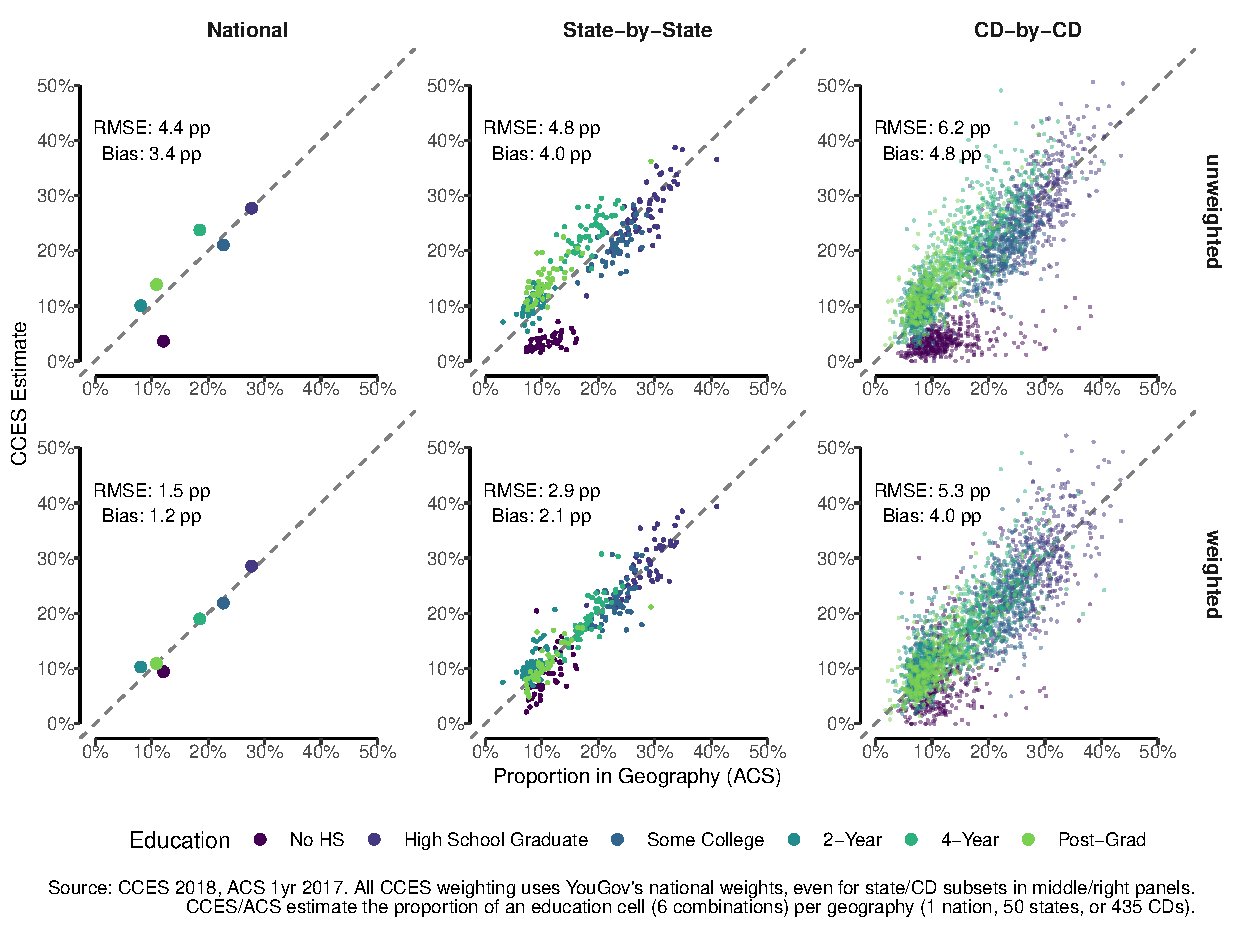
\includegraphics[width = \textwidth]{figures/educfrac-comparisons.pdf}
\end{figure}

\FloatBarrier

We next take a look not only at education, but the representativeness in terms of education-gender-age joint distributions. YouGov weights on first moments and (presumably two-way) interactions, so their weighted are not guaranteed to hold for three-way joint distributions.  Figure \ref{fig:cellfrac-ed-age-sex} shows those quantities of interest, proliferating the number of points to examine. We find:

\smallskip 
\begin{enumerate}
\item National estimates improve about as much as in Figure \ref{fig:cellfrac-ed} in ratio terms.
\item State estimates also improve somewhat, but not by much (8 percent reduction in RMSE, as opposed to 40 percent in the marginal distribution case).
\item District estimates do not improve, and its bias \emph{increases} slightly by 0.08 percentage points. The bias variance decomposition suggests that the variance has increased as well.
\item Some of the outliers in the state estimate suggests that the YouGov national weights up-weight some state-demographic cells in a way that makes them less representative of the state. 
\end{enumerate}

\begin{figure}[bt!h]
\centering
\caption{Representativeness of samples at different levels of geographies, education \(\times\) age \(\times\) gender fraction \label{fig:cellfrac-ed-age-sex}}
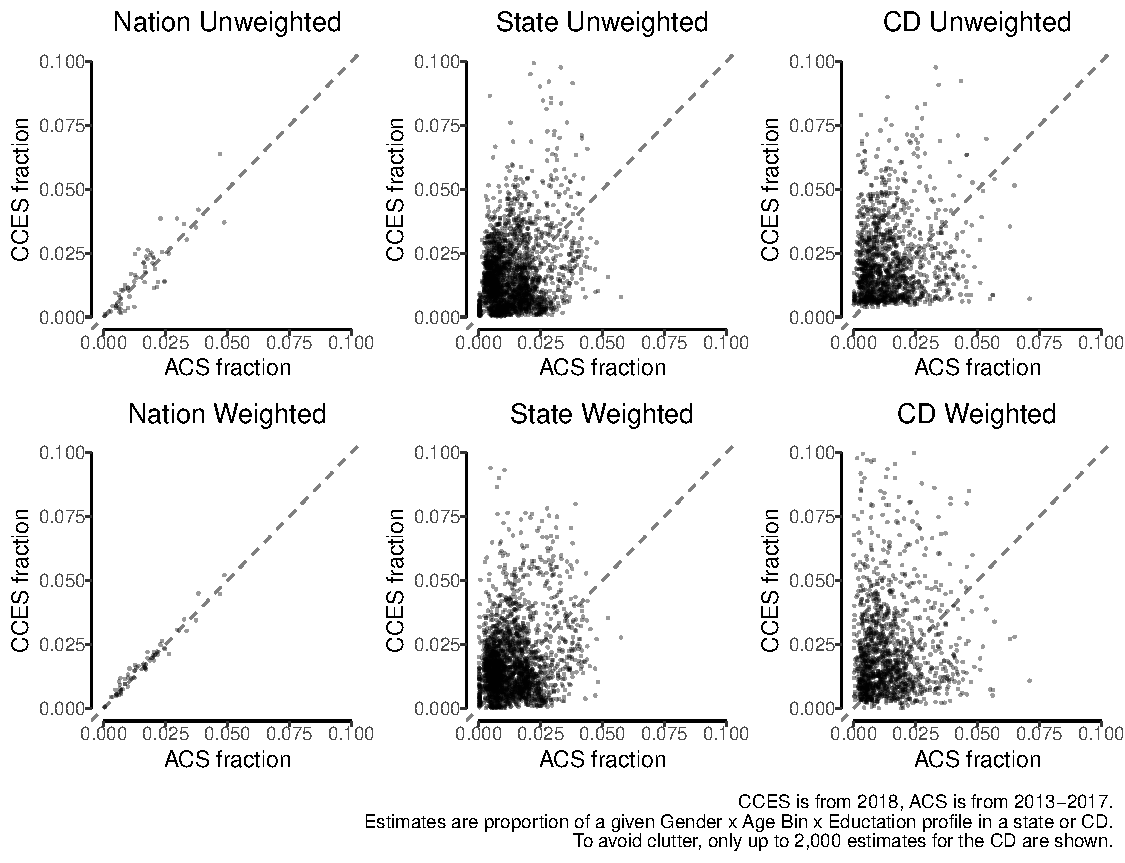
\includegraphics[width = \textwidth]{figures/cellfrac-comparisons.png}
\end{figure}

\FloatBarrier
\newpage

\section*{Custom Rim Weights}

Do weights that are specifically targeted to match on the state-specific moments improve representativeness? These weights must get the state-by-state marginal distributions exactly right by construction. How does it improve representativeness at larger or lower levels of aggregation? Figure \ref{fig:rim-comparisons} shows figures analogous to the prior figures:

\medskip
\begin{enumerate}
\item The rim weights coerce the marginal estimates to match the population targets, as expected.
\item Although each state subsample's weights is computed separately, its concatenation makes national estimates representatives too. 
\item At the smaller district level, the marginal estimates have also improved, and slightly outperform the YouGov weights.
\item However, rim weights do not necessarily improve representativeness of joint distributions. The bottom panel shows that those estimates are about as representative as those with YouGov weights, perhaps by reducing the variance.
\end{enumerate}

\FloatBarrier

\begin{figure}[!htbp]
\centering
\caption{Representativeness with custom state-by-state rim weights \label{fig:rim-comparisons}}
\includegraphics[width = \textwidth]{figures/educfrac-rim-comparisons.pdf}
\includegraphics[width = \textwidth]{figures/cellfrac-rim-comparisons.png}
\end{figure}

\FloatBarrier

\pagebreak


\appendix

\section{Introduction to Rake Weights and Iterated Weighting (rim weights)}

Post-stratification is the process of generating weights to coerce the weighted proportion of the sample to equal any given target distribution (it is called ``post'' because it occurs after the survey was fielded, instead of over-sampling low-propensity individuals during the survey). The method is very simple and was outlined in Deming and Stephan (1940). 

Index individuals by \(i \in \{1, ..., n\}\). Each individual has a scalar weight at iteration \(t\) as \(w^{(t)}_i\), and \(j \in \{1, ..., K\}\) categorical covariates \(\bm{X}_i\). For example, one grouping could be ``education'', which is a discrete variable with four levels (high school or less, 2-year college, college, or post-graduate). Denote the levels of group \(j\) by \(\ell \in \{1, ..., L_j\}\). 

For each grouping, there is a target distribution \[\bm{\pi}_j = \pi_{j1}, .... \pi_{KL_j}, ~~ \sum^{L_{j}}_{\ell = 1}\pi_{j\ell} = 1\] that we would like to hit. In parallel, there is an empirical proportion from the survey: \[\widehat{\bm{\pi}}_j = \widehat{\pi}_{j1},  ..., \widehat{\pi}_{jL}, ~~~\sum^{L_{j}}_{\ell = 1}\hat{\pi}_{g\ell} = 1.\]

These estimates are weighted averages of binary random variables, where th normalized weights at iteration \(t\) are applied as simple weighted means:
\[\bm{\widehat{\pi}}^{(t)}_{j\ell} = \frac{1}{n}\sum^n_{i=1}w_i^{(t)} \mathbf{1}(X_{ji} = \ell)\]

At each group \(j\), we update the weights simply by computing the ratio of target over actual for each level \(\ell\)
\begin{align}
r_{j\ell}^{(t+1)} = \frac{\pi_{j\ell}}{\widehat{\pi}^{(t)}_{j\ell}}
\end{align}
and apply these factors equally to all respondents for which \(X_{ji} = \ell\) that the sum of weights is \(n\),
\begin{align}
w_i^{(t+1)} \leftarrow \left(\sum^{L_j}_{\ell = 1}\mathbf{1}(X_{ji} = \ell)r_{j\ell}^{(t+1)}\right) \bigg / \underbrace{\left(\frac{1}{n}\sum^n_{i=1}\mathbf{1}(X_{ji} = \ell)r_{j\ell}^{(t+1)}\right)}_{\text{Normalizing factor}}
\end{align}

this will always set the proportion to the target because now for all \( \ell \in \{1, ..., L_j\},\)

\begin{align}
\frac{1}{n}\sum^n_{i=1}w_i^{(t+1)} \mathbf{1}(X_{ji} = \ell) =\frac{\pi_{j\ell}}{\widehat{\pi}^{(t+1)}_{j\ell}}\frac{1}{n}\sum^n_{i=1}\mathbf{1}(X_{ji} = 1) = \pi_{k\ell}
\end{align}

\paragraph{Convergence}
However, this does not necessarily guarantee that the weight \(w^{(t+1)}\) balances the sample moments for other groups \(k^{\prime}\). The algorithm cycles through each \(j \in \{1, ... K\}\). This constitutes one iteration.

At the each of iteration, the algorith assess total balance on typically a  squared loss:
\[SS^{(t+1)} = \sum^K_{j=1}\sum^{L_{j}}_{\ell = 1}\left(\frac{1}{n}\sum^n_{i=1}(w_i^{(t+1)}\mathbf{1}(X_{ji} = \ell)) - p_{j\ell}\right)\]

and stops if the sums of square is below some threhold, e.g. \(SS^{(t+1)} < 10^{-10}.\)


\paragraph{Limitations}
There are two limitations to this algorithm. The first is that users typically set a cap on the weights, e.g. \(w_{i} < 10\). The CCES caps weights at 15 for the commmon content (\(n = 60,000\)) and at 7 for team modules (\(n = 1,000\)). The second is easily expected from the fact that the main function has \(\widehat{p}_{j\ell}\) in the deominator, meaning it cannot be zero. This comes down to 

\[\sum^n_{i=1}\mathbf{1}(X_{j\ell} = 1) > 0, \forall j, \ell\]
i.e. that there is at least one observation for each level, in all groupings. This is essentially a limit on the number of dimensions one can match on. For example, if there are no Asian Americans over 65 years old in a sample of Vermont respondents, then the rim weighting cannot weight to race-age bin interactions.


\end{document}



 